\subsection{Controller}
Som de kan ses på figur \ref{fig:web}, er der en Controller, den indeholder alle PHP filer. Disse filer indeholder funktionen der anvendes til at sætte websiden op og hente/opdaterer data fra databasen. De følgende filer har hver deres opgave og disse vil blive beskrevet i følgende afsnit. Controller har følgende filerne som kan ses i tabel \ref{table:con_fil}. Hvis man ønsker at se filerne skal man gå ind under sourcekoden\footnote{Se bilag under Software\textbackslash www}.

\begin{table}[H]
\center
\setlength{\tabcolsep}{16pt}
\renewcommand{\arraystretch}{1.5}
	\begin{tabular}{ | >{\raggedright}p{3cm} | >{\raggedright\arraybackslash}p{9cm} | }
    \hline
    \rowcolor{lightgray} 
    \textbf{Kolonnenavn} 				& \textbf{Beskrivelse}  						\\ \hline
    \textit{mysql.php} 							& Opretter forbindelse til databasen											\\ \hline
    \textit{index.php}							& Bygger index/home siden til AVS												\\ \hline
    \textit{kar.php}							& Bygger kar siden til det kar man tilgår										\\ \hline
    \textit{create.php} 						& Opretter et kar, som bliver visualiseret i GUI'en og sat ind i databasen		\\ \hline
  	\textit{createSO.php} 						& Opretter en Sensor Ø som bliver visualiseret i GUI'en og sat ind i databasen	\\ \hline
   	\textit{delete.php} 						& Sletter et kar, både fra databasen og GUI'en									\\ \hline
   	\textit{deleteS.php}	 					& Sletter en Sensor Ø, både fra databasen og GUI'en							 	\\ \hline
   	\textit{edit.php}							& Redigere navnet på karet														\\ \hline
   	\textit{updateData.php}						& Opdaterer de indtastede data i karet											\\ \hline
   	\textit{auto\_refresh\_kar.php}				& opdaterer de aflæste date og er sammentidlig en fil der bliver opdateret hvert sekund \\ \hline
\end{tabular}
\caption{Beskrivelser af php filer under Controller}
\label{table:con_fil}
\end{table}
I følgende er der nogle af filerne der bliver beskrevet mere detaljeret, for at illustrer hvordan de påvirker gui'en og databasen.


\subsubsection{index}
Under template mappen ligger der en \textit{index.html} fil, som visualiserer vores webside for \gls{AVS}, denne side indeholder alle kar, men da html kun er front og antallet af kar er ukendte er der lavet noget php kode til at hente alle kar og deres informationerne hver gang man opdaterer siden, . her er smarty anvendt så man kan lave en lykke i html som så viser alle kar.\\\\
\begin{minipage}{.5\textwidth}
\begin{lstlisting}[caption=index.php]
	.
	.
	.
	.
// Get all Kar
$kars = getKars($conn);

// Render page
$smarty = new Smarty;
$smarty->assign('kars', $kars);
	.
	.
	.
	.
	.
\end{lstlisting}
\end{minipage}% This must go next to `\end{minipage}`
\begin{minipage}{.5\textwidth}
\begin{lstlisting}[caption=index.html]
	.
	.
{foreach $kars as $kar}
	<li class="list-group-item">
	<div class="row">
		<div class="col-xs-4">
			<a href="kar.php?id={$kar.id}">
				{$kar.name}
			</a>
		</div>
	.
	.																		
{/foreach}
	.
	.
\end{lstlisting}
\end{minipage}

Det gør at denne liste kan blive genereret ud fra databasen så man kan tilgå alle kar, disse kar linker til en ny side, som er baseret på karets id, se figur \ref{fig:index}. 
\begin{figure}[H]
    \centering
    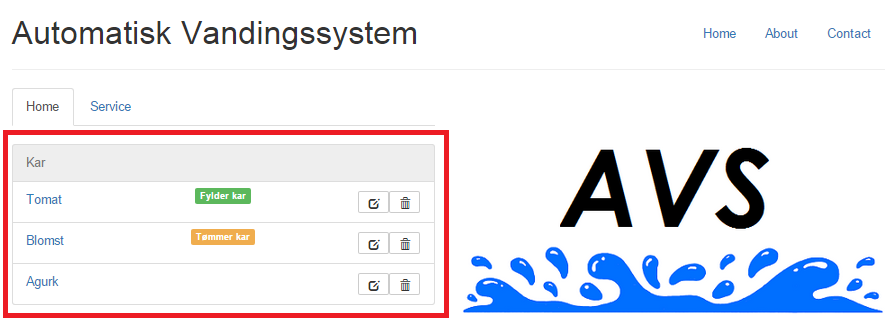
\includegraphics[width=0.9\textwidth]{SoftwareArkitektur/GUI/Controller/photo/index.PNG}
    \caption{AVS websiden}
    \label{fig:index}
\end{figure}

\subsubsection{kar}
Under template mappen ligger der en \textit{kar.html} fil, som visualisere websiden for hver enkle kar, baseret på deres id. den laver også en liste over Sensor Øerne, ved at anvende samme teknik som da man skulle have listen over kar, se figur \ref{fig:so}.  

\begin{figure}[H]
    \centering
    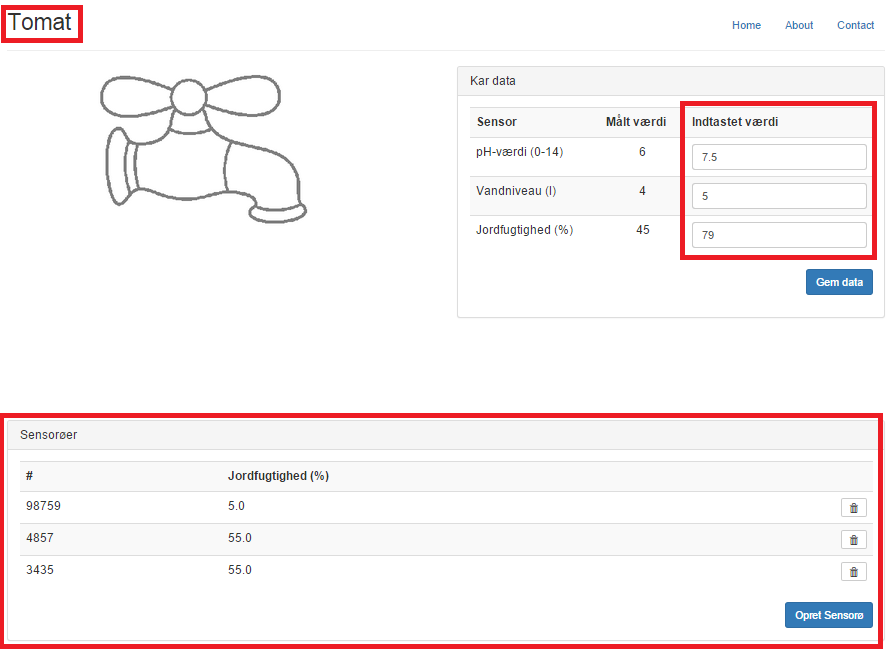
\includegraphics[width=0.9\textwidth]{SoftwareArkitektur/GUI/Controller/photo/so.PNG}
    \caption{Del af kar siden, for karet med navn Tomat}
    \label{fig:so}
\end{figure}

Desuden er der nogle knapper, som kalder en funktion så snart de bliver trykket på. Knapperne er på karet personlige side, som set på figur \ref{fig:knap}
\begin{figure}[H]
    \centering
    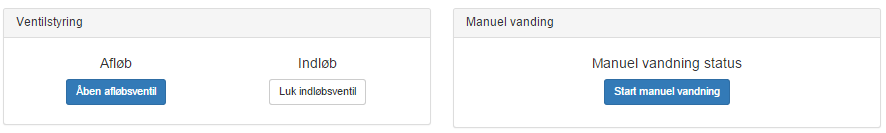
\includegraphics[width=0.9\textwidth]{SoftwareArkitektur/GUI/Controller/photo/knap.PNG}
    \caption{knapper til karet}
    \label{fig:knap}
\end{figure}

For at give et eksempel på hvordan de kalder en funktion ser vi på start manuel vanding. Den knap har php kode

\begin{lstlisting}[caption=index.php]
	.
	.
$id = $_POST['id'];
	.
	.
if(array_key_exists('MWSTART',$_POST)){
    $client->connect();
	//Manual watering start
	$client -> MWStart($id);
} 
	.
	.
\end{lstlisting}

Hvis koden til html filen har navnet 'MWSTART', og knappen bliver trykket ned, bliver der oprettet forbindelse til socket serveren og den få en besked om at manuel vanding skal startes. Knappens navn og udsende bliver sat alt efter hvilken status manuel vanding har, og den status kan aflæses på karets informationer fra databasen.


\subsubsection{auto\_refresh\_kar} 
Som nævnt tidligere er der anvendt jQuery AJAX metoder, som kan bruges til at udveksle data med en server og opdatere dele af en webside uden at genindlæse hele siden. Dette er lavet så de aflæste data bliver opdateret hvert 5 sekund og knapperenes status bliver opdateret hvert sekund. Da dette er lavet over de ting der er markeret på figur \ref{fig:auto}.  

\begin{figure}[H]
    \centering
    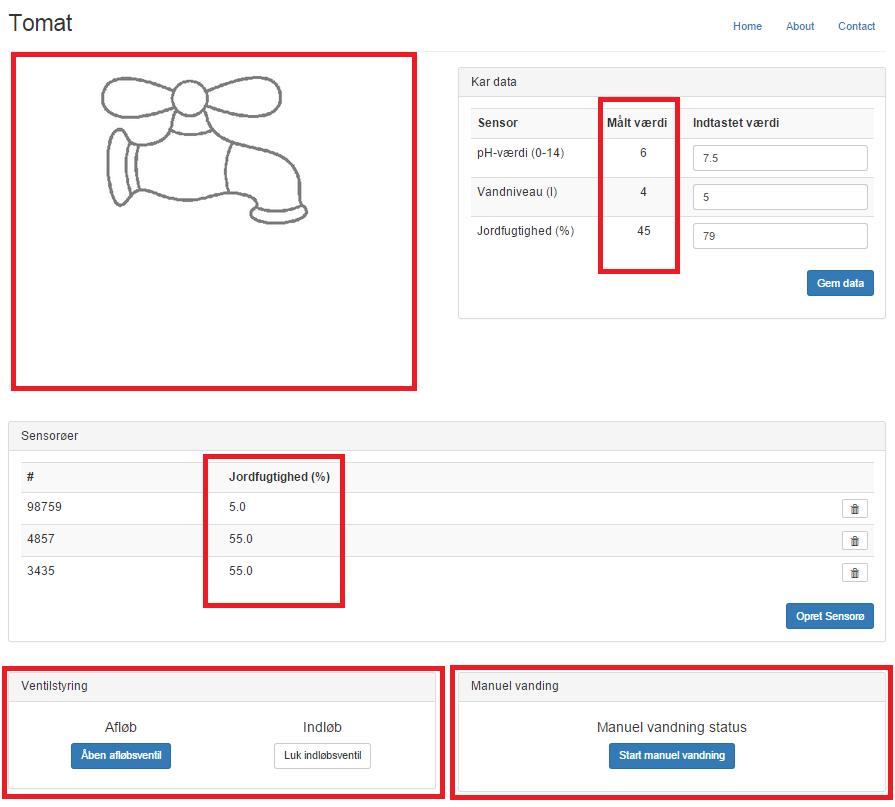
\includegraphics[width=0.9\textwidth]{SoftwareArkitektur/GUI/Controller/photo/auto.PNG}
    \caption{Dele auto\_refresh\_kar påvirker}
    \label{fig:auto}
\end{figure}

Da det går meget igen hvordan koden er implementeret for at opdaterer knapperne og de forskellige data, bliver det kun gennemgået for knappen manuel vanding. Selve processen for at få manuel vandingsstatus kan ses på følgende sekvens diagram.

\begin{figure}[H]
    \centering
    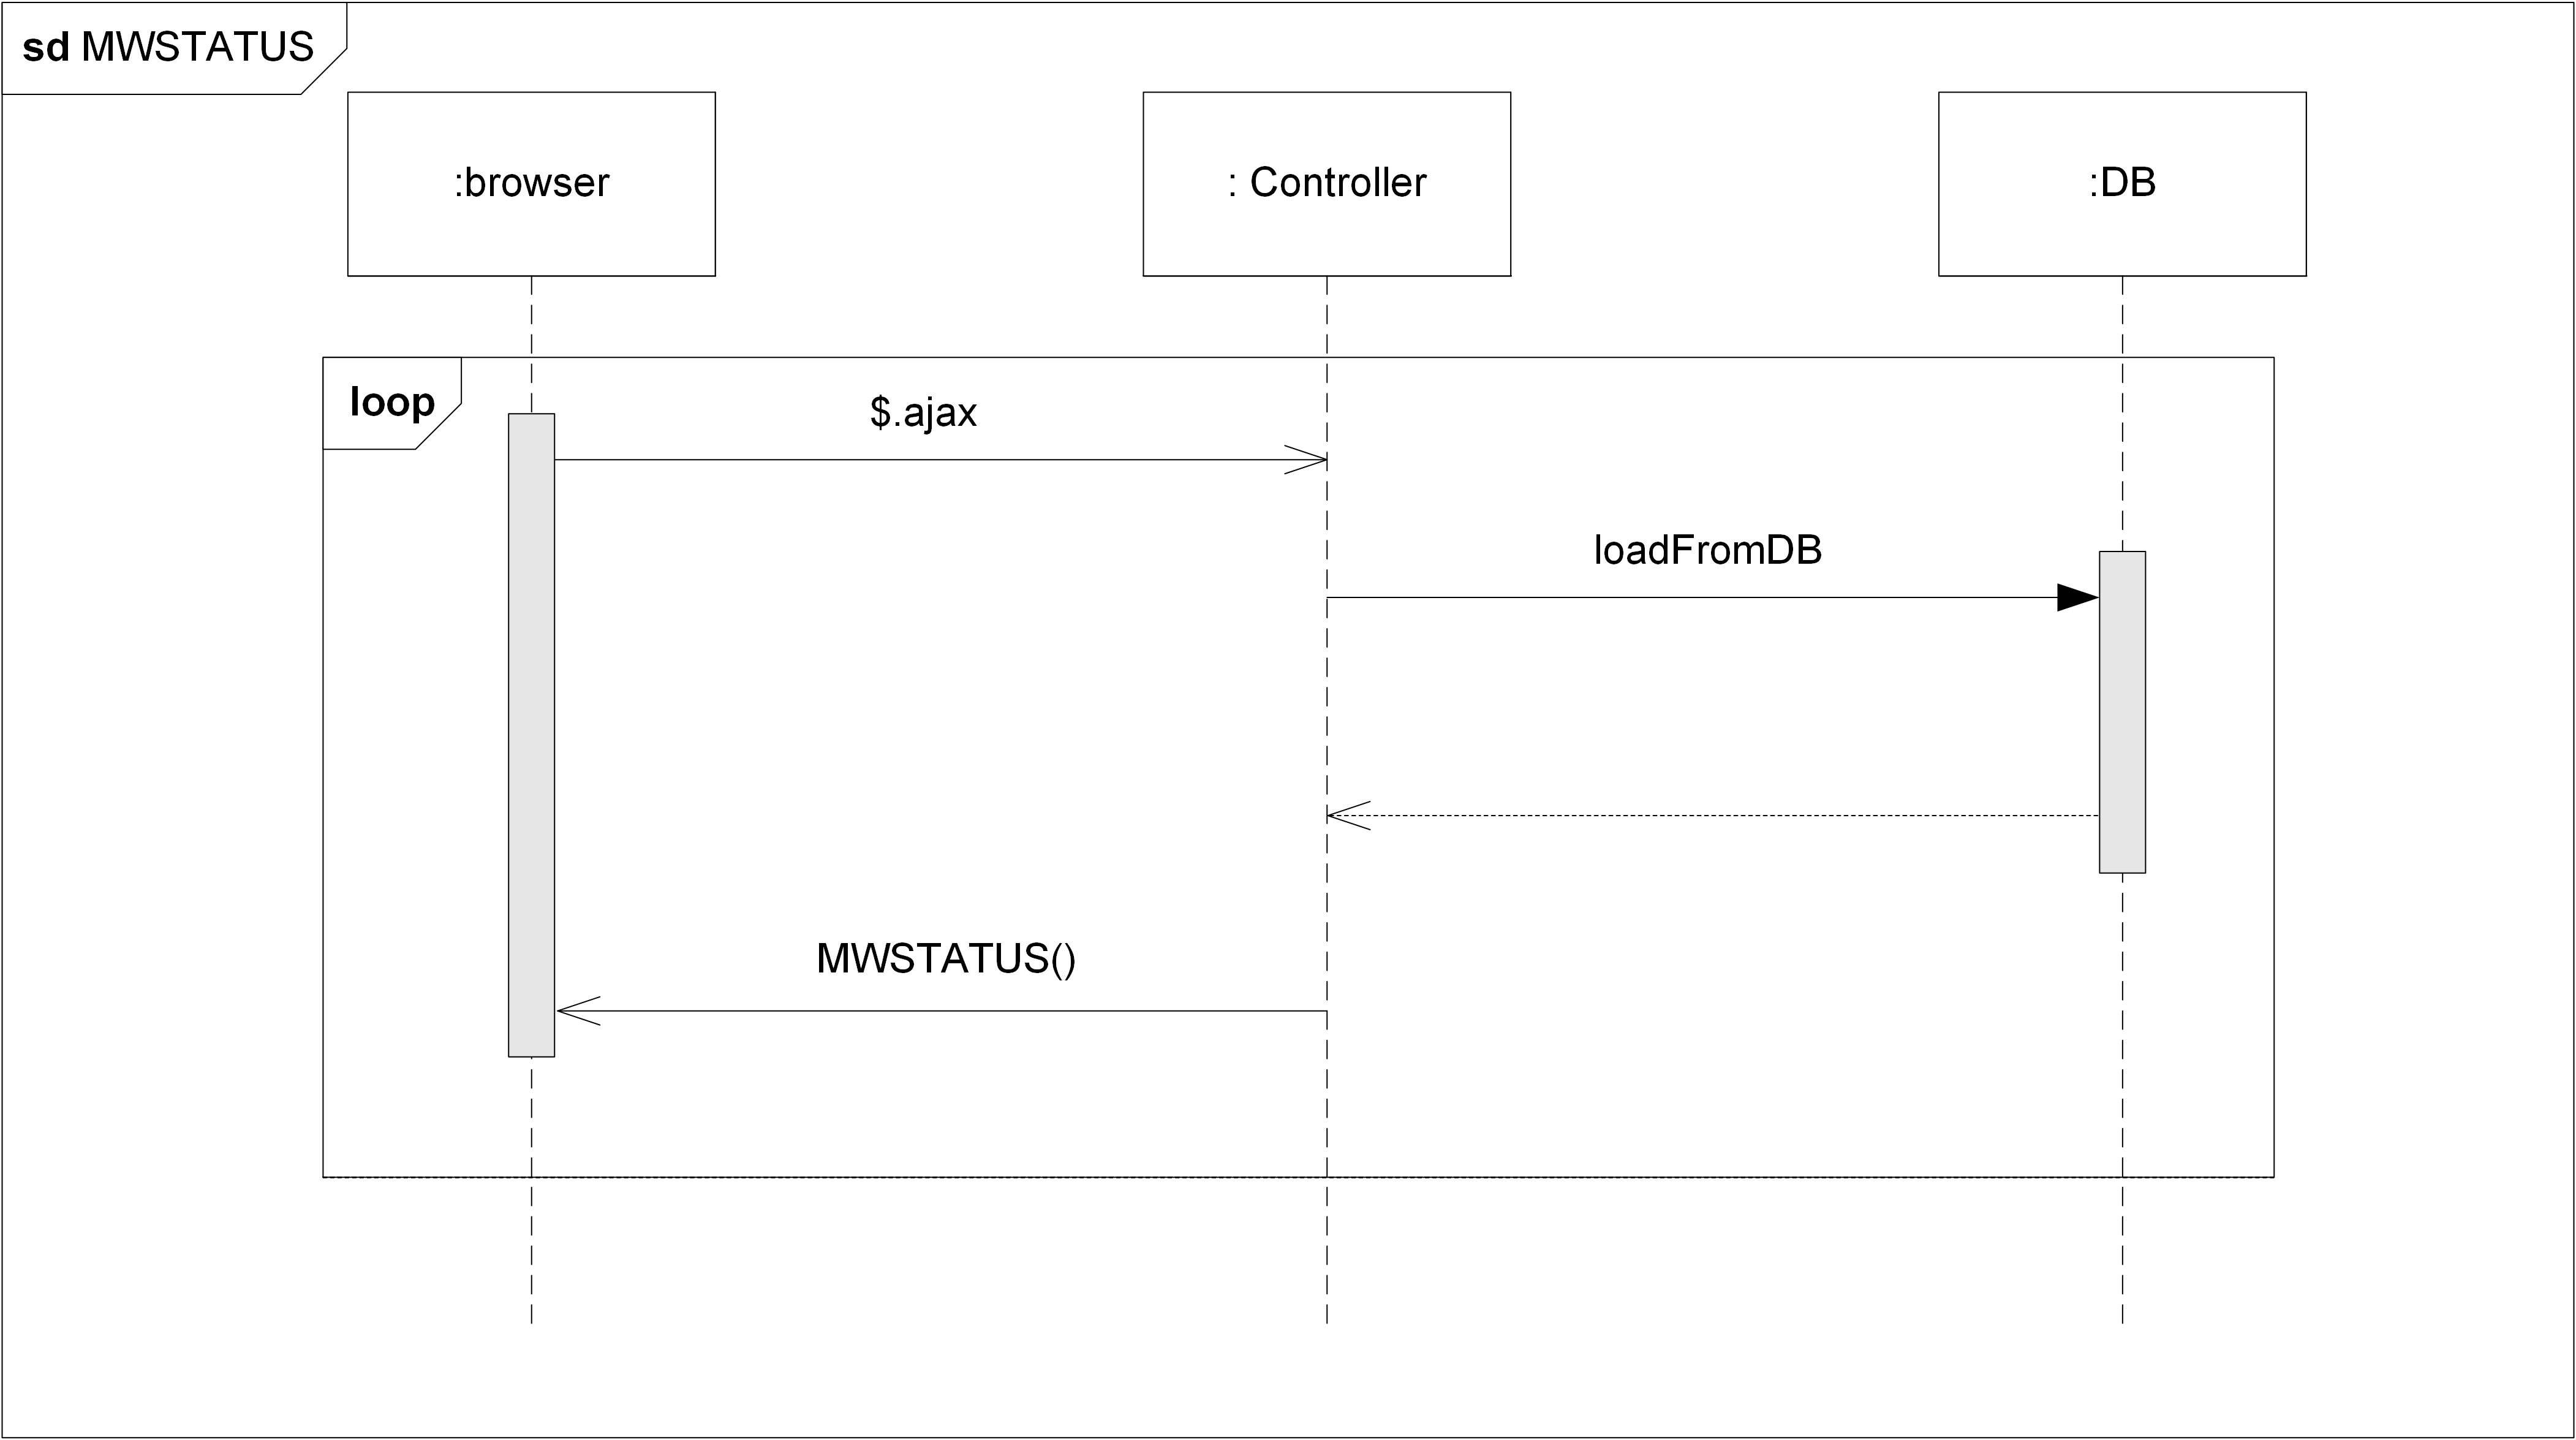
\includegraphics[width=0.8\textwidth]{SoftwareArkitektur/GUI/Controller/photo/sd_mwstatus.PNG}
    \caption{Sekvensdiagram for manuel vanding status}
    \label{fig:knap}
\end{figure}


sekvens diagrammet illustrerer, at ved at bruge ajax kan man lave et loop det sender en request hvert sekund og modtager en ønskede data. Koden for manuel vandings knappen er implementeret med JavaScript, html og php således: \\
\begin{minipage}{.5\textwidth}
\begin{lstlisting}[caption=JavaScript]
	.
	.
	.
function refreshStatuses(){
$.ajax({
  url: "auto_refresh_kar.php",
  method: "GET",
  data: { id: {$kar->id} },
  dataType: "json",
  success: function( data ) {
	if(data.mwstatus == 1){
	  $("#MWSTATUS" )
	  .html("Stop manuel vandning")
	  .removeClass('btn btn-primary btn-md')
	  .addClass('btn btn-default btn-md')
	  .attr("name","MWSTOP");
	  $("#image").attr("src","medie/VHV.png");
	}else{
	  $("#MWSTATUS" )
	  .html("Start manuel vandning")
	  .removeClass('btn btn-default btn-md')
	  .addClass('btn btn-primary btn-md')
	  .attr("name","MWSTART");
	  $("#image").attr("src","medie/VH.png");
	}
		.
		.
		.	
			
  }
 })
}
		.
		.
		.
	
$(function() {							
  refreshStatuses();
  refreshKarSensorData();
  setInterval(refreshStatuses, 1000); 		
  setInterval(refreshKarSensorData, 5000);	
});
	.
	.
	.
\end{lstlisting}
\end{minipage}% This must go next to `\end{minipage}`
\begin{minipage}{.5\textwidth}
\begin{lstlisting}[caption=html]
	.
	.
<div class="panel-body text-center">
  <h4> Manuel vandning status</h4>
  <form action="kar.php?id={$kar->id}" method="post">
    <button id="MWSTATUS" type="submit" name="" value="1" class=""></button>
  </form>
</div>
	.
	.
\end{lstlisting}
\begin{lstlisting}[caption=php]
	.
	.
$id = $_GET['id'];

// Kar connection
$kar = new Kar($conn);

// Load kar with $id
if(!$kar->loadFromDB($id))
{
	die("Ikke fundet!");
}
	.
	.
$statusses = array(
	'mwstatus' => (int) $kar->MWSTATUS,
	'ivalvestatus' => (int) $kar->IVALVESTATUS,
	'ovalvestatus' => (int) $kar->OVALVESTATUS,
	'ph' => (double) $ph,
	'volumen' => (int) $volumen,
	'humidity' => (int) $humidity,
	'sensorOeData' => $soData,
);
	
	
json_encode($statusses);
	.
	.
	.
\end{lstlisting}
\end{minipage}

I javaScript koden, bliver funktion på linje 37-42, kaldt hver gang siden bliver opdateret. og derefter bliver funktionerne knappernes status opdateret hvert sekund og kar sensor dataene bliver opdateret hvert 5 sekund. 
\\\\
På linje 4-32 bliver de funktionen der opdatere knapperne implementeret, den bruger GET metoden. Den tager det tilhørende kar id, som bliver defineret i linje 3 i php koden. 
\\\\
Id'et bliver lavet til at finde de værdier der er til karet med tilhørende kar id. derefter bliver de gemt i et array (linje 15-23), hvor den bliver lavet til en JSON repræsentation af værdien på linje 26. 
\\\
Tilbage til javaScript koden, kan værdierne fra array nu anvendes. På linje 11 bliver det undersøgt om manuel vanding er i gang og hvis det er tilfældet bliver alt koden på linje 12-17 kørt. 
\\\\
på linje 12 i javaScript koden tager vi fat i det html kode der har id "MWSTATUS", som kan ses på linje 6 i html koden. her bliver "name", "class" og teksten sat alt efter hvad manuel vandings status er. 
\\\\
Så i tilfælde af at en starter manuel vanding, bliver dens status ændret i databasen og knappen bliver opdateret uden brugeren skal genopfriske siden. 



 